\setAuthor{Mihkel Pajusalu}
\setRound{lõppvoor}
\setYear{2010}
\setNumber{G 3}
\setDifficulty{2}
\setTopic{Elektriahelad}

\prob{Päikesepaneel}
Joonisel on kujutatud päikesepaneeli läbiva voolu sõltuvus klemmipingest.
Määrake paneeli klemmidega ühendatud koormise takistus, mille korral on koormisel eralduv
võimsus maksimaalne.

\begin{center}
	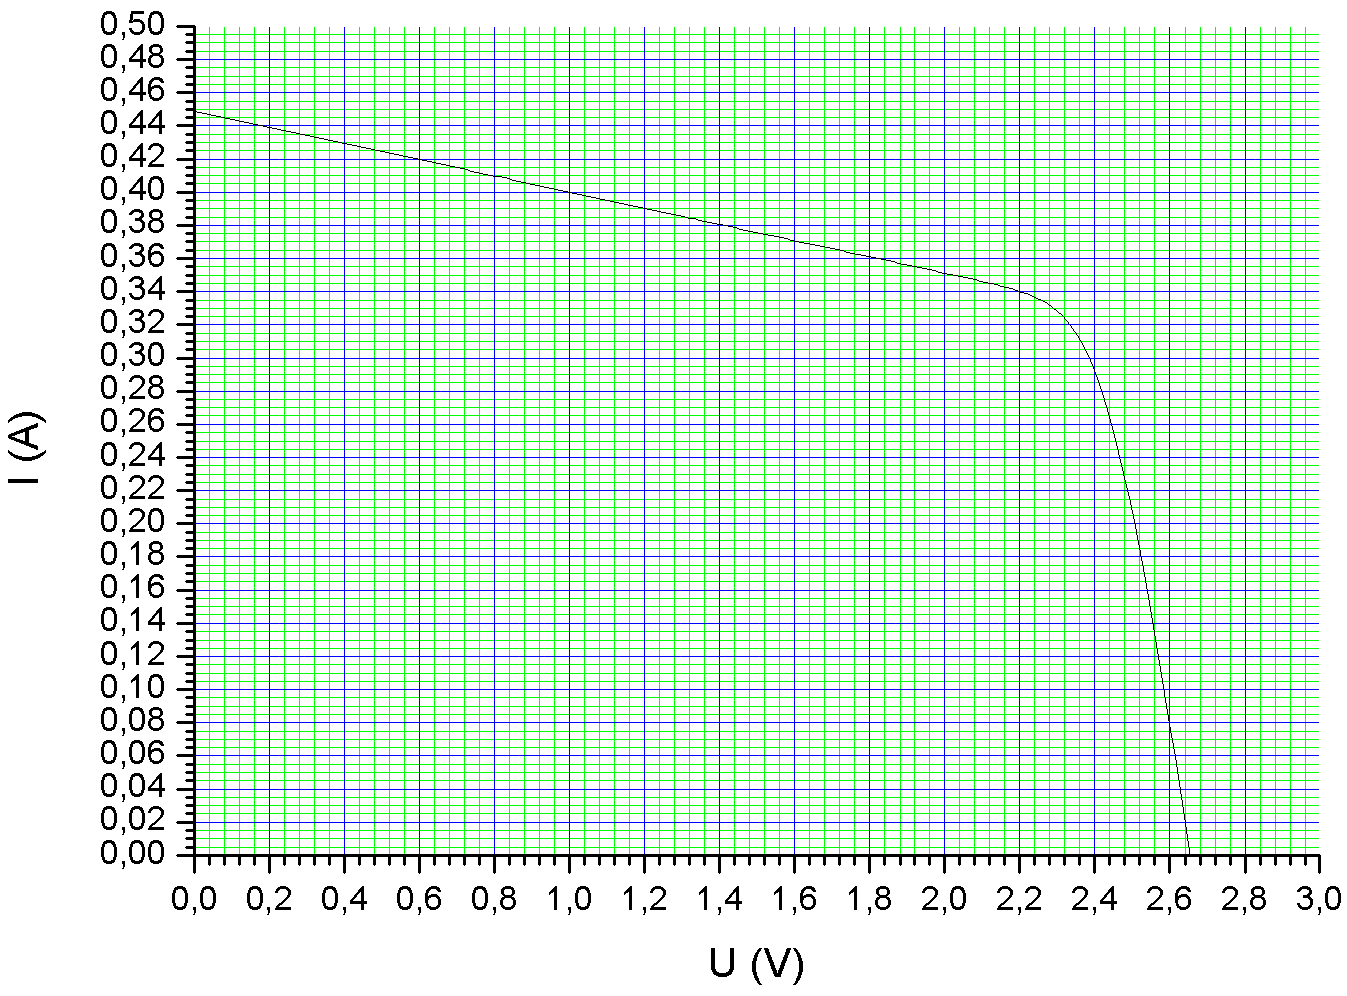
\includegraphics[width=0.9\linewidth]{2010-v3g-03-paneel_yl.png}
\end{center}

\hint
Koormisel eralduv võimsus on pinge ja voolu korrutis. Seega on vaja graafikult leida $x$- ja $y$-koordinaadi korrutise maksimum.

\solu
Koormisel eralduv võimsus avaldub kui $UI$. Peame leidma punkti graafikul, mil antud avaldis on maksimaalne. Toore jõuga lähenedes saab graafikult erinevate punktide jaoks võimsuse välja arvutada ja ligikaudu maksimaalse võimsuse määrata. Saame $U\idx{max} \approx \SI{2.28}{V}$, $I\idx{max}\approx \SI{0.33}{A}$. Seega vastav koormise takistus on
\[
R = \frac{U_\mathrm{max}}{I_\mathrm{max}} \approx \SI{6.9}{\ohm}
\]


\begin{center}
	\vspace{-0.1cm}
	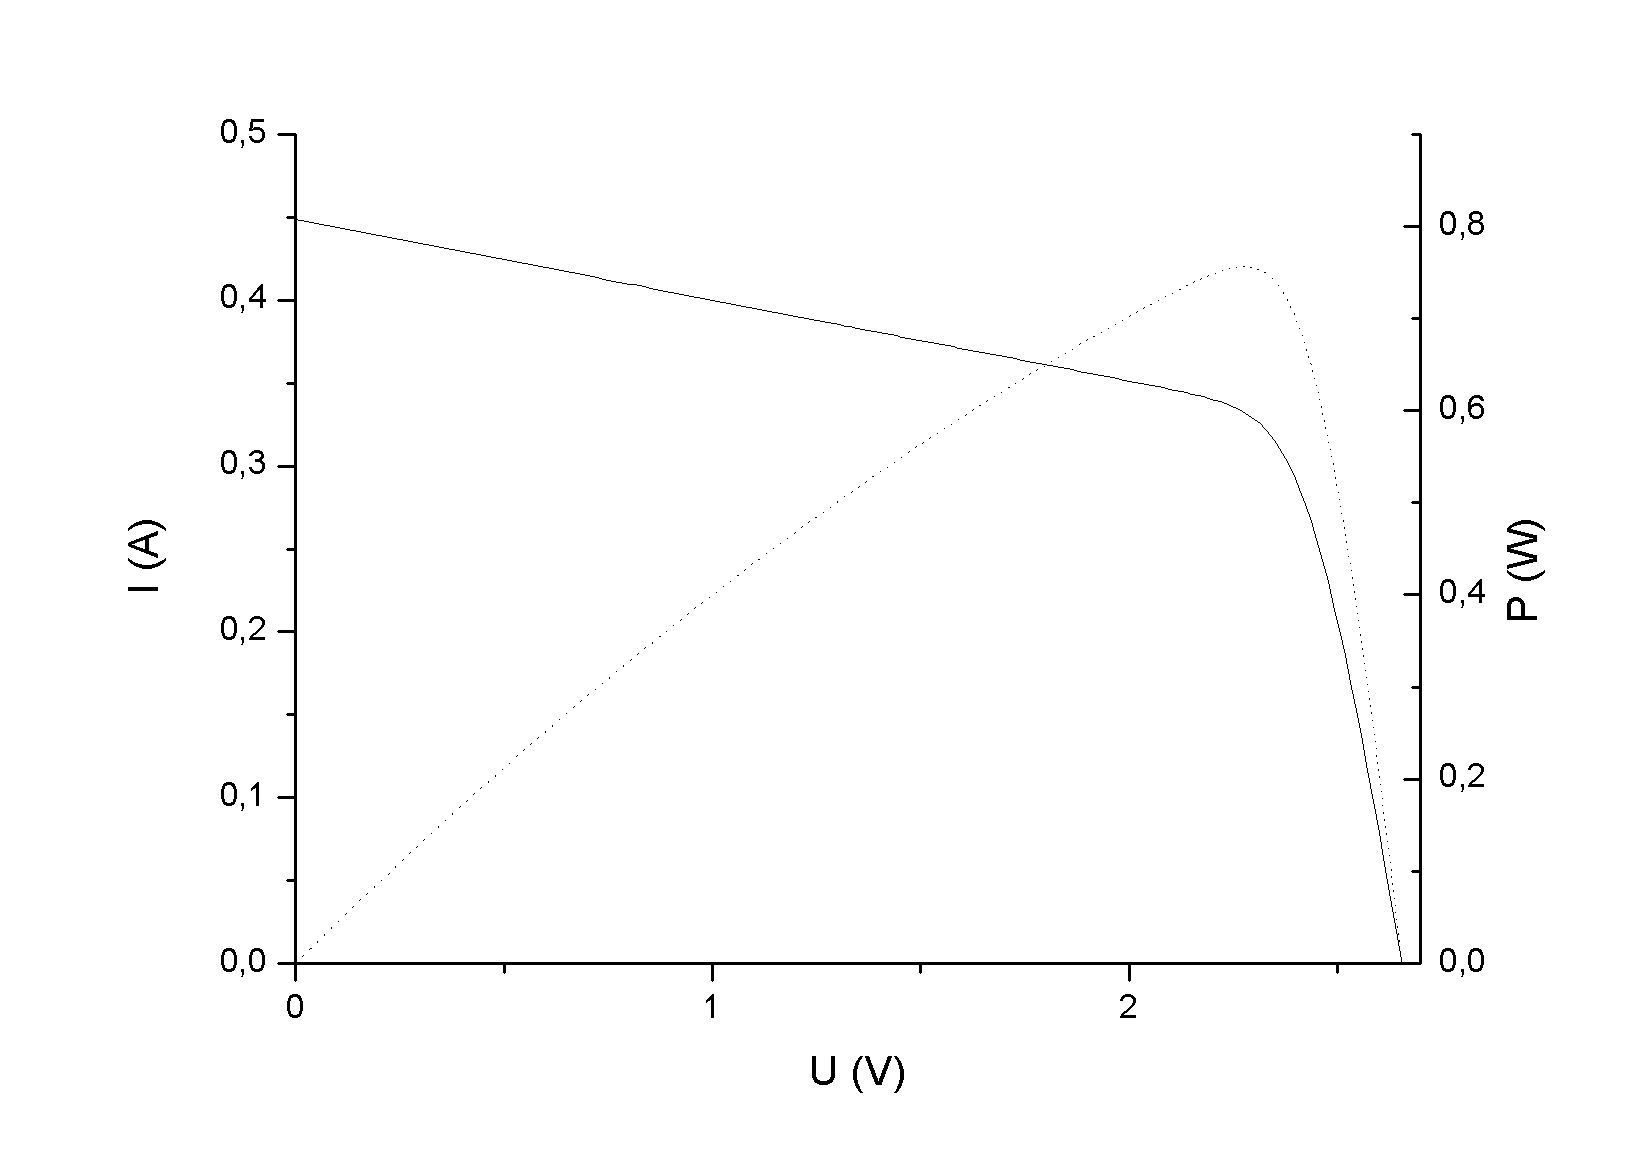
\includegraphics[width=0.8\linewidth]{2010-v3g-03-paneel_lah.png}
\end{center}

\textit{Alternatiivne lahendus}\\

\begin{center}
	\hspace{-0.1cm}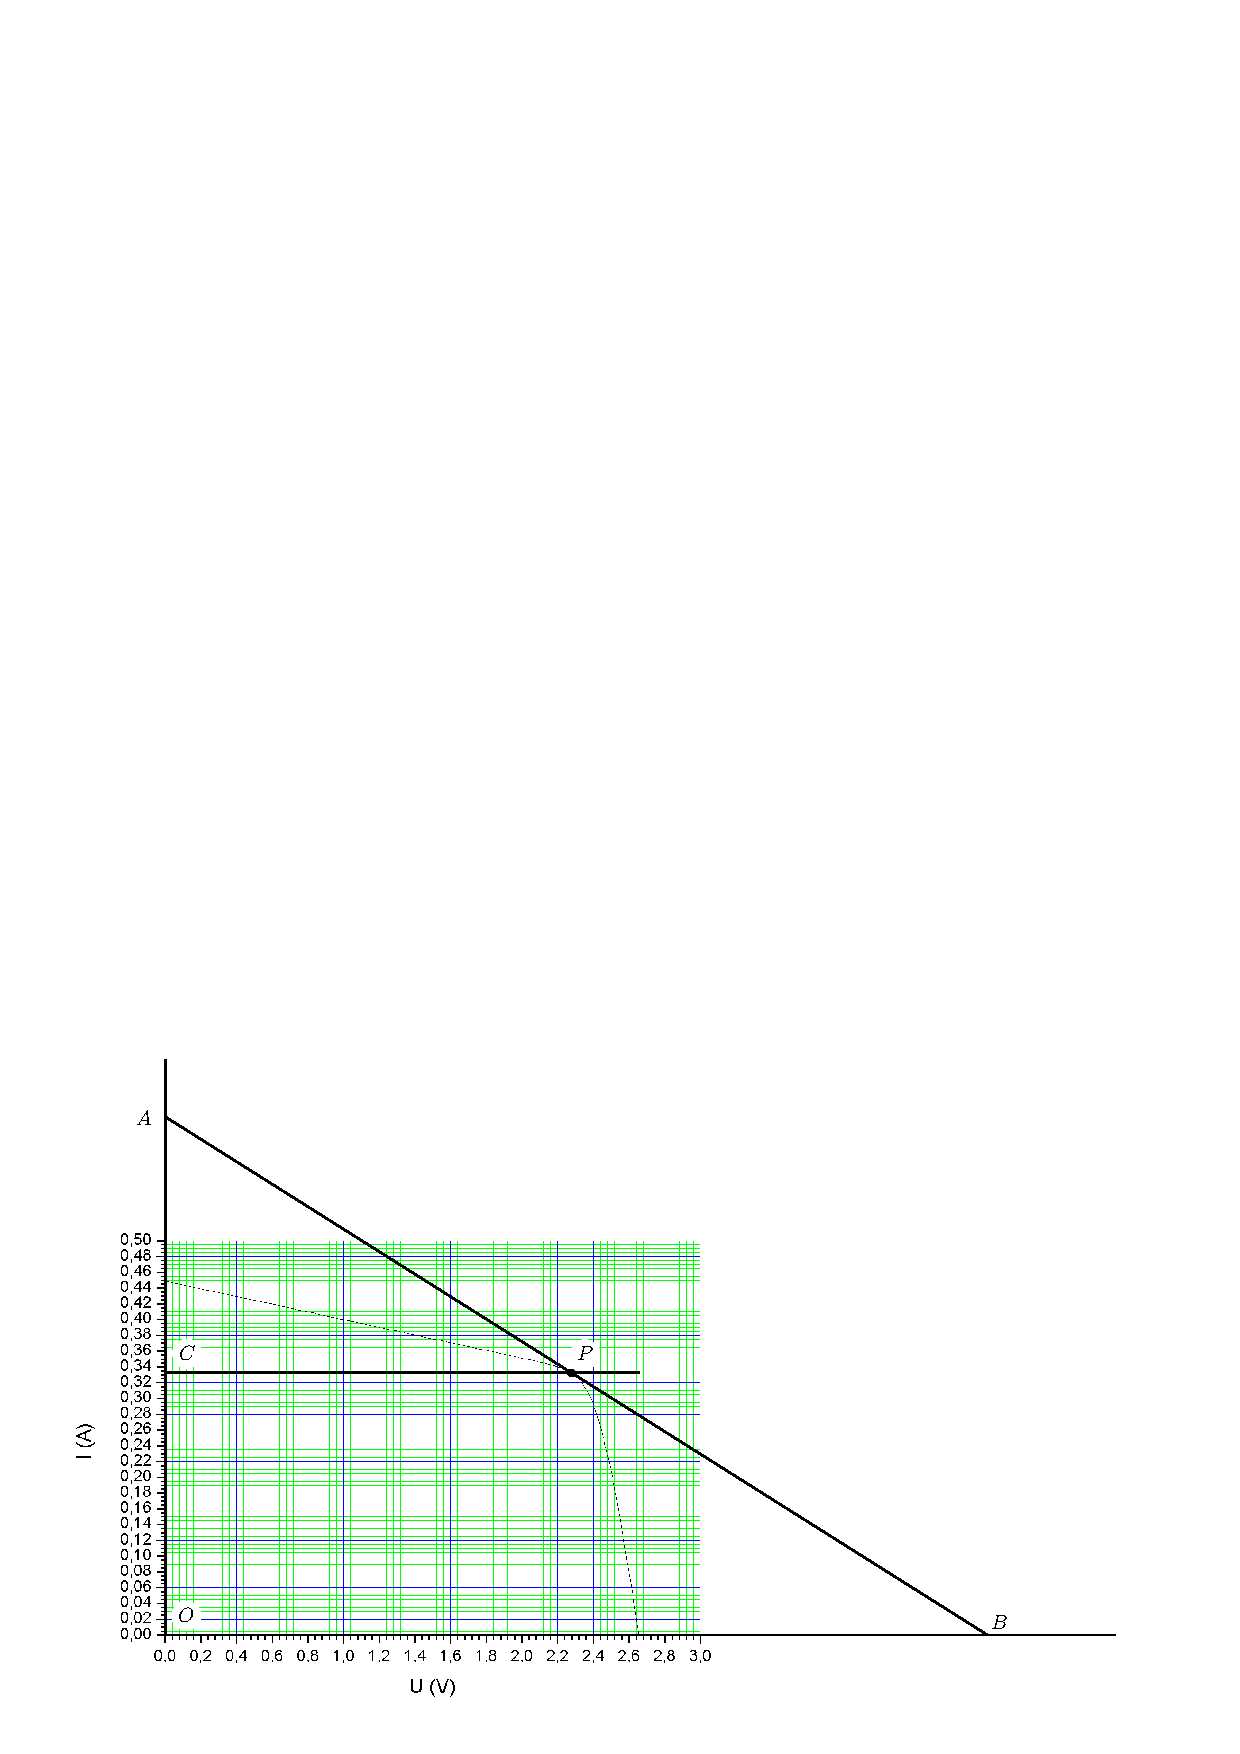
\includegraphics[width=130mm]{2010-v3g-03-joonis_paneel_lah_2}
\end{center}

Võimsus $N = UI$ on maksimaalne, kui võimsuse tuletis pinge järgi on null. Seega,
\[
\D N = \D (UI) = \D UI + U\D I = 0,
\]
ehk
\[
I + U\frac{\D I}{\D U} = 0,
\]
kus $\D I/\D U$ on graafiku tõus. Vaatleme vastavaid suurusi graafiku puntkis $P$. Joonise tähistustes, $|OC| = I$, $|CP| = U$ ja
\[
\frac{|OA|}{|OB|} =
\frac{|CA|}{|CP|} = -\frac{\D I}{\D U}.
\]
Järelikult, kui me tahame, et
$P$ oleks otsitav võimsuse maksimumi punkt, peab kehtima
\[
|OC| - |CP|
\frac{|CA|}{|CP|} = 0 \implies |OC| = |CA| \implies |AP| = |PB|.
\]
Joonlauaga veidi otsides pole sellist punkti $P$ raske leida. Vastus on muidugi sama, mis esimeses lahenduses.
\probend